\section{Yuyan}

Please present main results on manifold ...

\subsection{Manifold Learning}
Suppose there a dataset $\mathbf X =(\mathbf x_1,...,\mathbf x_n)$ and each $\mathbf x_i\in \mathbb R^d$. In many  practical problem, the $\mathbf x_i$ locates on a low dimension manifold $\mathcal M$ in $\mathbb R^d$. The goal of Manifold Learning is to find the parameter coordinate of $\mathcal M$, so we can present the points $\mathbf x_1,...,\mathbf x_n$ in a essential form.
\subsubsection{Isomap}
The main idea of isomap is to keep the geodesic distance of $\mathcal M$ during dimensionality reduction.


The Figure \ref{fig:isomapmnist} is the effect of Isomap for MNist, it shows different digit in the MNist dataset is separable.
%\begin{figure}
	%\centering
	%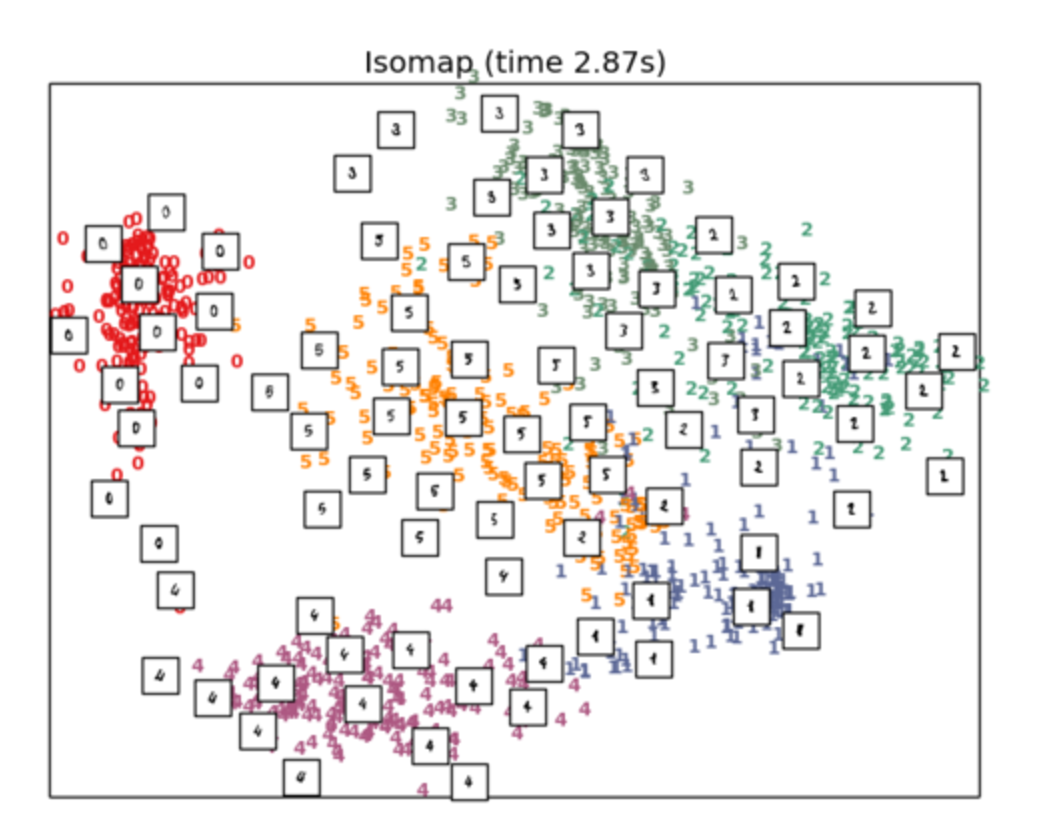
\includegraphics[width=0.7\linewidth]{../figures/IsomapMnist}
	%\caption{The effect of Isomap for MNist}
	%\label{fig:isomapmnist}
%\end{figure}
